\documentclass[compress]{beamer}\usepackage[]{graphicx}\usepackage[]{xcolor}
% maxwidth is the original width if it is less than linewidth
% otherwise use linewidth (to make sure the graphics do not exceed the margin)
\makeatletter
\def\maxwidth{ %
  \ifdim\Gin@nat@width>\linewidth
    \linewidth
  \else
    \Gin@nat@width
  \fi
}
\makeatother

\definecolor{fgcolor}{rgb}{0.345, 0.345, 0.345}
\newcommand{\hlnum}[1]{\textcolor[rgb]{0.686,0.059,0.569}{#1}}%
\newcommand{\hlstr}[1]{\textcolor[rgb]{0.192,0.494,0.8}{#1}}%
\newcommand{\hlcom}[1]{\textcolor[rgb]{0.678,0.584,0.686}{\textit{#1}}}%
\newcommand{\hlopt}[1]{\textcolor[rgb]{0,0,0}{#1}}%
\newcommand{\hlstd}[1]{\textcolor[rgb]{0.345,0.345,0.345}{#1}}%
\newcommand{\hlkwa}[1]{\textcolor[rgb]{0.161,0.373,0.58}{\textbf{#1}}}%
\newcommand{\hlkwb}[1]{\textcolor[rgb]{0.69,0.353,0.396}{#1}}%
\newcommand{\hlkwc}[1]{\textcolor[rgb]{0.333,0.667,0.333}{#1}}%
\newcommand{\hlkwd}[1]{\textcolor[rgb]{0.737,0.353,0.396}{\textbf{#1}}}%
\let\hlipl\hlkwb

\usepackage{framed}
\makeatletter
\newenvironment{kframe}{%
 \def\at@end@of@kframe{}%
 \ifinner\ifhmode%
  \def\at@end@of@kframe{\end{minipage}}%
  \begin{minipage}{\columnwidth}%
 \fi\fi%
 \def\FrameCommand##1{\hskip\@totalleftmargin \hskip-\fboxsep
 \colorbox{shadecolor}{##1}\hskip-\fboxsep
     % There is no \\@totalrightmargin, so:
     \hskip-\linewidth \hskip-\@totalleftmargin \hskip\columnwidth}%
 \MakeFramed {\advance\hsize-\width
   \@totalleftmargin\z@ \linewidth\hsize
   \@setminipage}}%
 {\par\unskip\endMakeFramed%
 \at@end@of@kframe}
\makeatother

\definecolor{shadecolor}{rgb}{.97, .97, .97}
\definecolor{messagecolor}{rgb}{0, 0, 0}
\definecolor{warningcolor}{rgb}{1, 0, 1}
\definecolor{errorcolor}{rgb}{1, 0, 0}
\newenvironment{knitrout}{}{} % an empty environment to be redefined in TeX

\usepackage{alltt}

% Load ttbeamer template depending on operating system
\usepackage{ifplatform}
\ifwindows
  \usepackage{M:/pc/Dokumenter/ttbeamer}
\fi
\iflinux
  \usepackage{/home/tony/uio/pc/Dokumenter/ttbeamer}
\fi
\ifmacosx
  \usepackage{/Users/tctan/uio/pc/Dokumenter/ttbeamer}
\fi

\title{Lecture 3 - Statistics Review and Item Statistics}
\author[]{Tony Tan \\\vspace{6pt} {\em{University of Oslo}} }
\date{Friday, 21 October 2022}
\IfFileExists{upquote.sty}{\usepackage{upquote}}{}
\begin{document}



\begin{frame}[fragile]
  \titlepage
\end{frame}


\begin{frame}[fragile]
  \frametitle{Today's session}
    \begin{itemize}
      \item Review of concepts: expectation, variance, covariance and correlation
      \item Illustrate statistical principles
      \item Define some useful notation
      \item Discuss different types of statistics and their interpretation for various types of item and test data
    \end{itemize}
\end{frame}


\section{Statistics review}

\begin{frame}[fragile]
  \frametitle{Sums, products, and sets}
    Let $a_1, a_2, \dots, a_K$ be a set of constants. The \ttemph{sum} of these constants is written
      \[ \sum_{k = 1}^K a_k = a_1 + a_2 + \dots + a_K. \]
    The \ttemph{product} of these constants is written
      \[ \prod_{k = 1}^K a_k = a_1 \times a_2 \times \dots \times a_K. \]

      In this notation, $k$ is an \ttemph{index variable} which takes integer values from 1 to the number $K$.

    A \ttemph{set} is denoted as $\mathcal{A} = \{1, 2, \dots, K\}$. We say that ``3 belongs to set $\mathcal{A}$'', and write $3 \in \mathcal{A}$.
\end{frame}


\begin{frame}[fragile]
  \frametitle{Expected value}
    Let $X$ be a \ttemph{discrete} random variable (R.V.) taking $k$ different values with probabilities $p_1, \dots, p_k$. The \ttemph{expected value} of $X$ is
      \[ \E{X} = \sum_{i = 1}^k x_i\, p_i. \]

      Let $Y$ be a \ttemph{continuous} R.V. with support $(a, b)$ and density $f(\cdot)$. The expected value of $Y$ is
      \[ \E{Y}=\int_a^b y\, f(y)\, \dd y. \]

      The expected value is a \ttemph{parameter} often denoted by $\mu$. We can interpret it as the long-run average value of the random variable under repeated sampling. Expected values can be infinite or undefined.
\end{frame}


\begin{frame}[fragile]
  \frametitle{Expected value: Example}
    Let $X$ be a discrete R.V. which can take values $x_1 = 0$ or $x_2 = 1$ with corresponding probabilities $p_1 = 0.4$ and $p_2 = 0.6$. The expected value of $X$ is
    \begin{equation*}
      \begin{aligned}
        \E{X} &= \sum_{i = 1}^2 x_i\, p_i\\
              &= 0 \times 0.4 + 1 \times 0.6\\
              &= 0.6.
      \end{aligned}
    \end{equation*}
\end{frame}


\begin{frame}[fragile]
  \frametitle{Linearity of the expected value}
    For a number of R.V.s $X_1, \dots, X_k$, the expectation of their sum is the sum of their expectations
      \[ \E{X_1 + \dots + X_k} = \E{X_1} + \dots + \E{X_k}, \]
    and for constants $a_1, \dots, a_k$
      \[ \E{a_1 X_1 + \dots + a_k X_k} = a_1 \E{X_1} + \dots + a_k \E{X_k}. \]

    That it, expectation is transparent to \ttemph{linear} operations.
\end{frame}


\begin{frame}[fragile]
  \frametitle{Linearity of the expected value: Example}
    Let $X_1$ and $X_2$ be two random variables, where $\E{X_1} = 0.6$ and $\E{X_2} = 0.4$. The expected value of their sum
    \begin{equation*}
      \begin{aligned}
        \E{X_1 + X_2} &= \E{X_1} + \E{X_2}\\
                      &= 0.6 + 0.4 \\
                      &= 1.
      \end{aligned}
    \end{equation*}

    Consider constants $a_1 = 1$ and $a_2 = 2$. The expected value of the linear combination
    \begin{equation*}
      \begin{aligned}
        \E{a_1X_1 + a_2X_2} &= a_1 \E{X_1} + a_2 \E{X_2} \\
        & = 1 \times 0.6 + 2 \times 0.4 \\
        & = 1.4.
      \end{aligned}
    \end{equation*}
\end{frame}


\begin{frame}[fragile]
  \frametitle{The $k$-th moment}
    Let $X$ be a discrete R.V. that can take $l$ different values with probabilities $p_1, \dots, p_l$. The $k$-th moment of $X$ is
      \[ \E{X^k} = \sum_{i=1}^l x_i^k p_i. \]

    Let $Y$ be a continuous R.V. with support $(a, b)$ and density $f(\cdot)$. The $k$-th moment of $Y$ is
      \[ \E{Y^k} = \int_a^b y^k f(y)\, \dd y. \]
\end{frame}


\begin{frame}[fragile]
  \frametitle{The $k$-th moment: Example}
    Let $X$ be a discrete R.V. that can take values
      \[ x_1 = 0,\ x_2 = 1,\ \text{or } x_3 = 2 \]
    with corresponding probabilities
      \[ p_1 = 0.2,\ p_2 = 0.3,\ \text{and } p_3 = 0.5. \]
    The 4th moment of $X$ is
    \begin{equation*}
      \begin{aligned}
        \E{X^4} &= 0^4 \times 0.2 + 1^4 \times 0.3 + 2^4 \times 0.5 \\
                &= 0 + 0.3 + 8\\
                &= 8.3.
      \end{aligned}
    \end{equation*}
\end{frame}


\begin{frame}[fragile]
  \frametitle{The sample mean}
    Let $x_1, \dots, x_n$ denote the sample. The \ttemph{sample mean} $\bar{x}$ is computed as
      \[ \bar{x}=\frac{1}{n}\sum_{i=1}^n x_i. \]

    The sample mean is often used as an \ttemph{estimator} of the parameter $\mu$.
\end{frame}


\begin{frame}[fragile]
  \frametitle{Variance and standard deviation}
    \ttemph{Variances} measure the dispersion of the data. For a R.V. $X$ with expected value $\mu$,
      \[ \V{X} = \mathbb{E} \left[ (X - \mu)^2 \right] = \E{X^2} - \mu^2. \]

    The variance is a parameter often denoted by $\sigma^2$.

    The \ttemph{standard deviation} $\sigma$ is the positive square root of the variance.
\end{frame}


\begin{frame}[fragile]
  \frametitle{Properties of variance}
    Let $X$ and $Y$ be two R.V.s. The variances of their sum and difference are
      \[ \V{X \pm Y} = \V{X} + \V{Y} \pm 2\,\cov{X}{Y}. \]

    For constants $a$ and $b$,
      \[ \V{aX \pm bY} = a^2 \V{X} + b^2 \V{Y} \pm 2\,ab\,\cov{X}{Y}. \]
\end{frame}


\begin{frame}[fragile]
  \frametitle{Sample variance}
    For a sample $x_1, \dots, x_n$, we can estimate their \ttemph{sample variance} $s^2$
      \[ s^2 = \frac{1}{n-1} \sum_{i=1}^n (x_i - \bar{x})^2. \]
  Dividing by $n - 1$ is required in order to obtain the \ttemph{unbiased} sample variance.

  Example: We observe
    \[ 5, 6, 9, 3, 20. \]
  The sample mean is
    \[ (5 + 6 + 9 + 3 + 20) / 5 = 8.6. \]
  The unbiased sample variance is
  \[ [(5 - 8.6)^2 + (6 - 8.6)^2 + (9 - 8.6)^2 + (3 - 8.6)^2 + (20 - 8.6)^2] / (5 - 1) = 45.3. \]
\end{frame}


\begin{frame}[fragile]
  \frametitle{Covariance}
    Consider two R.V.s $X$ and $Y$. The \ttemph{covariance} is a measure of the degree to which $X$ and $Y$ are interrelated
      \begin{equation*}
        \cov{X}{Y} = \mathbb{E} \left\{
              \left[ X - \E{X} \right]
              \left[ Y - \E{Y} \right]
            \right\}.
      \end{equation*}

      Covariance is a parameter that can be estimated by the sample covariance. For matching-pair samples $(\m{x},\m{y})=(x_i, y_i)$, their \ttemph{sample covariance} is
        \begin{equation*}
          \hat{\mathrm{Cov}}(\m{x},\m{y}) = \frac{1}{n-1} \sum_{i=1}^n
            \left[ x_i - \bar{x} \right]
            \left[ y_i - \bar{y} \right].
        \end{equation*}
\end{frame}


\begin{frame}[fragile]
  \frametitle{Properties of covariance}
    From the definition of covariance, we have
    \begin{equation*}
      \begin{aligned}
        \cov{X}{Y} &= \mathbb{E} \left[ (X - \E{X}) (Y - \E{Y}) \right] \\
        &= \mathbb{E} \left[ XY - X\E{Y} - \E{X}Y + \E{X}\E{Y} \right] \\
        &= \E{XY} - \E{X}\E{Y} - \E{X}\E{Y} + \E{X}\E{Y} \\
        &= \E{XY} - \E{X}\E{Y}.
      \end{aligned}
  \end{equation*}
\end{frame}


\begin{frame}[fragile]
  \frametitle{Covariance and independence}
    Since
      \[ \cov{X}{Y} = \E{XY} - \E{X}\E{Y}, \]
    if $X$ and $Y$ are \ttemph{independent},
      \[ \cov{X}{Y} = \E{XY} - \E{X}\E{Y} = 0. \]

    However, $\cov{X}{Y} = 0$ does \ttemph{not} necessarily imply that $X$ and $Y$ are \ttemph{independent}.
\end{frame}


\begin{frame}[fragile]
  \frametitle{Correlation}
    \begin{itemize}
      \item The magnitude of the covariance is difficult to interpret on its own because its value depends on the scale of the R.V.s $X$ and $Y$.
      \item A standardised measure, the correlation, can be used as a measure of the magnitude of the \ttemph{linear relationship} between two R.V.s.
    \end{itemize}

    The \ttemph{Pearson correlation} is
      \[ \rho_{X,Y}=\frac{\cov{X}{Y}}{\sigma_X\sigma_Y}, \]
    where $\sigma_X$ and $\sigma_Y$ are the standard deviations of $X$ and $Y$ respectively.

    Note that $-1 \leq \rho_{X,Y} \leq 1$.
\end{frame}


\begin{frame}[fragile]
  \frametitle{Pearson correlation measures a linear relationship}
    

    \begin{figure}[!htpb]
      \begin{center}
\begin{knitrout}
\definecolor{shadecolor}{rgb}{0.969, 0.969, 0.969}\color{fgcolor}
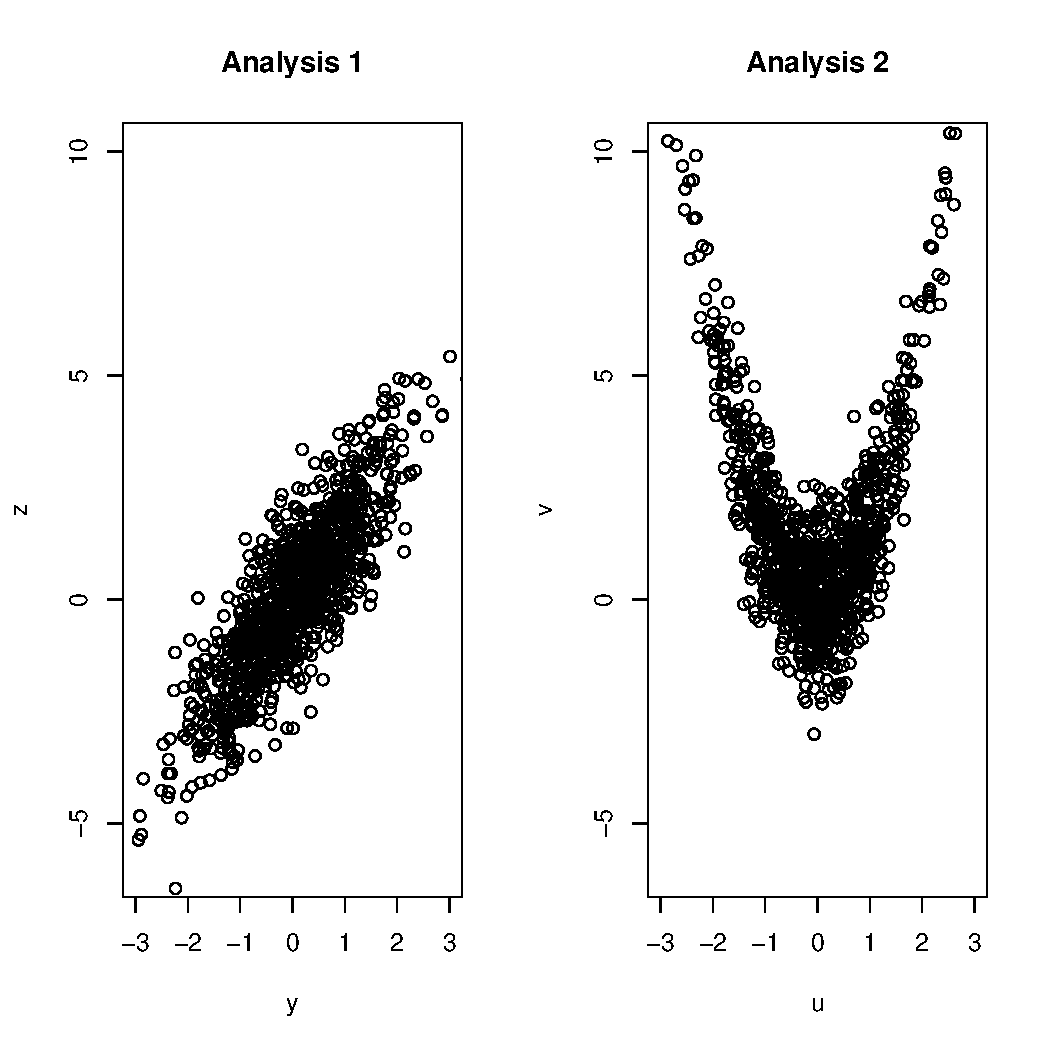
\includegraphics[width=\maxwidth]{figure/plot21-1} 
\end{knitrout}
      \end{center}
    \end{figure}
\end{frame}


\begin{frame}[fragile]
  \frametitle{Pearson correlation measures a linear relationship}
\begin{knitrout}
\definecolor{shadecolor}{rgb}{0.969, 0.969, 0.969}\color{fgcolor}\begin{kframe}
\begin{alltt}
  \hlkwd{cor}\hlstd{(y, z)}
\end{alltt}
\begin{verbatim}
## [1] 0.8440646
\end{verbatim}
\begin{alltt}
  \hlkwd{cor}\hlstd{(u, v)}
\end{alltt}
\begin{verbatim}
## [1] -0.09752877
\end{verbatim}
\end{kframe}
\end{knitrout}
\end{frame}


\begin{frame}[fragile]
  \frametitle{Statistics}
    \begin{itemize}
      \item Statistics can be viewed as the methods by which we draw conclusions from \ttemph{incomplete} information
      \item We design the data collection by considering statistical principles
      \item We utilize statistical methods when analysing the data
      \item We use statistical \ttemph{inference} to accept or reject \ttemph{hypotheses} or add knowledge to a body of scientific results
      \item All empirical research utilises statistical methods and principles
    \end{itemize}
\end{frame}


\begin{frame}[fragile]
  \frametitle{Parameters, estimators, and estimates}
    \begin{itemize}
      \item The ``truth'': The parameter (e.g. $\mu$)
      \item How we learn about the truth: The estimator (e.g. $\hat{\mu}$)
      \item What we learn from the truth: The estimate (e.g. $\hat{\mu}_{\mathrm{obs}}$)
    \end{itemize}
\end{frame}


\begin{frame}[fragile]
  \frametitle{Standard deviation and standard error}
    Note the difference in these two concepts
      \begin{itemize}
        \item Standard deviation: The square root of the variance of a \ttemph{random variable} $\sqrt{\V{Y}}$ or of a population parameter $\sqrt{\V{\theta}}$
        \item Standard error: The square root of the variance of an \ttemph{estimator} $\sqrt{\V{\hat{\theta}}}$
      \end{itemize}
\end{frame}


\begin{frame}[fragile]
  \frametitle{Confidence intervals}
    \begin{itemize}
      \item A 95\% confidence interval $(a, b)$ for a parameter $\theta$ means that the parameter $\theta$ is covered by such an interval 95\% of the time if the sampling would be repeated infinitely.
      \item The confidence interval does \ttemph{not} mean that the parameter has probability 0.95 of being in the interval. (cf. credible interval)
      \item In practice, we \ttemph{estimate} a confidence interval and that interval either covers or does not cover the true parameter.
    \end{itemize}
\end{frame}


\begin{frame}[fragile]
  \frametitle{Exercise}
    \begin{itemize}
      \item We observed the heights of 50 randomly selected UiO students.
      \item The sample mean was 173.4 cm and the sample standard deviation 15.5 cm.
      \item The standard error of the mean can be calculated by $\mathrm{se}(\bar{x}) = \sqrt{s^2/n}$, where $s^2$ is the sample variance and $n$ is the sample size.
    \end{itemize}

    Estimate a 95\% confidence interval for the population mean height and interpret the results.
\end{frame}

\begin{frame}[fragile]
  \frametitle{Solution}
    \begin{itemize}
      \item We observe $\bar{x}=173.4$ cm and $\mathrm{se}(\bar{x}) = 15.5\ \text{cm} / \sqrt{50} \approx 2.2$ cm.
      \item We note that the statistic $(\bar{x} - \mu) / \text{se}(\bar{x})$ follows the $t$-distribution with 49 degree of freedom.
      \item We calculate $t(49)_{(0.025)} \approx -2.0$ and construct the confidence interval for $\mu$ as
      \[ \left( \bar{x} - 2.0 \times 2.2,\ \bar{x} + 2.0 \times 2.2 \right) = (169.0, 177.8). \]
    \end{itemize}

    That is, if we were to repeat the sampling infinitely many times, the true value $\mu$ would be covered by such an estimated interval 95\% of the time.
\end{frame}


\begin{frame}[fragile]
  \frametitle{Notation}
    \begin{itemize}
      \item $\mu$ --- expected value
      \item $\E{X}$ --- expected value of $X$
      \item $\sigma^2$ --- variance
      \item $\V{X}$ --- variance of $X$
      \item $\cov{X}{Y}$ --- covariance of $X$ and $Y$
      \item $\rho$ --- correlation
    \end{itemize}
\end{frame}


\begin{frame}[fragile]
  \frametitle{Bias, variance and mean squared error of an estimator}
    For an estimator $\hat{\theta}$ of a parameter $\theta$, the \ttemph{bias} is defined as
      \[ \text{Bias} \left( \hat{\theta} \right) = \E{\hat{\theta} - \theta}. \]

    If $\text{Bias} \left( \hat{\theta} \right) = 0$, we say that the estimator $\hat{\theta}$ is an \ttemph{unbiased estimator} of $\theta$.

    The estimator also has a variance
      \[ \V{\hat{\theta}} = \mathbb{E} \left\{ \left[ \hat{\theta} - \E{\hat{\theta}} \right]^2 \right\}. \]

    We often consider the \ttemph{mean squared error} (MSE) of an estimator
      \[ \text{MSE} \left( \hat{\theta} \right) = \mathbb{E} \left[ \left( \hat{\theta} - \theta \right)^2 \right]. \]

    It can be shown that $\text{MSE} \left( \hat{\theta} \right) = \V{\hat{\theta}} + \left[ \text{Bias} \left( \hat{\theta} \right) \right]^2$.
\end{frame}


\begin{frame}[fragile]
  \frametitle{Distributions}
    \begin{itemize}
      \item $X \sim \mathcal{N}(\mu, \sigma^2)$ --- $X$ follows a normal distribution with mean $\mu$ and variance $\sigma^2$
      \item $X \sim t(\nu)$ --- $X$ follows a $t$-distribution with $\nu$ degrees of freedom
      \item $X \sim \chi^2(\nu)$ --- $X$ follows a $\chi^2$-distribution with $\nu$ degrees of freedom
    \end{itemize}
\end{frame}

\begin{frame}[fragile]
  \frametitle{R.V.s and their observations}
    \begin{itemize}
    \item The textbook defines upper-case letters as \ttemph{random variables} and lower-case letters as \ttemph{observations} from a sample.
    \item $X_j$ denotes the $j$-th item score on a test and is a random variable
    \item $x_{ji}$ denotes the score obtained on item $j$ for an individual $i$ and is an observation rather than a random variable
    \end{itemize}
\end{frame}

\begin{frame}[fragile]
  \frametitle{Mean vectors and covariance matrices}
    We can have vector-value random variables. We can consider the joint distribution of two variables $X, Y$.
      \begin{equation*}
        \m{\mu} =
          \begin{bmatrix}
            \E{X} \\
            \E{Y}
          \end{bmatrix},\ %
        \m{\Sigma} =
          \begin{bmatrix}
            \V{X}       &\cov{X}{Y} \\
            \cov{Y}{X}  &\V{Y}
          \end{bmatrix}.
      \end{equation*}
\end{frame}


\section{Item statistics}

\begin{frame}[fragile]
  \frametitle{Expected value of binary scores}
    \begin{itemize}
      \item If the item score $X_j$ can take values 0 or 1, it is a \ttemph{binary item}
      \item The sample mean $\frac{1}{n}\sum_{i=1}^n x_{ji}$ can be used to compute an estimate of $\mu_j = \E{X_j}$
      \item Since this is a binary item, the parameter $\mu_j=\E{X_j}$ can be interpreted as defining the probability $\pi_j$ of a randomly selected individual answering the item correctly
    \end{itemize}
\end{frame}


\begin{frame}[fragile]
  \frametitle{Variance of binary scores}
    For a random variable $X_j$ defined such that
      \[ \p{X_j = 1} = \pi_j,\ \text{and } \p{X_j = 0} = 1 - \pi_j, \]
    we have
      \[ \E{X_j} = \pi_j, \]
    and
      \[ \E{X_j^2} = 0^2 \times (1 - \pi_j) + 1^2 \times \pi_j= \pi_j. \]

    Since $\V{X_j} = \E{X_j^2} - \left[ \E{X_j} \right]^2$,
      \[ \V{X_j} = \pi_j - \pi_j^2 = \pi_j ( 1 - \pi_j ). \]

    To estimate the variance of a binary variable we can simply calculate the sample mean $\hat{p}_j$ and obtain
      \[ \hat{\mathrm{Var}} \left( X_j \right) = \hat{p}_j ( 1 - \hat{p}_j ). \]

    Note that this is a \ttemph{biased} estimator of the variance, since it is divided by $n$ instead of $n - 1$.
\end{frame}


\begin{frame}[fragile]
  \frametitle{Covariances of binary scores}
    The sample covariance between two sets of observations $\{x_i\}$ and $\{y_i\}$ is
      \[ s_{xy} = \frac{1}{n - 1} \sum_{i=1}^n(x_i - \bar{x})(y_i - \bar{y}). \]

    For binary variables $X_j$ and $X_k$, this expression reduces to 
      \[ s_{jk} = p_{jk} - p_jp_k, \]
    where $p_{jk}$ denotes the relative frequency of the event $\{X_j = 1, X_k = 1\}$, which can be estimated from the sample.
\end{frame}


\begin{frame}[fragile]
    \frametitle{Exercise: Variance and covariance of binary scores}
      We observe the following frequencies from a sample $\{x_i\}$, $\{y_i\}$:

      \begin{center}
        \begin{tabular}{|c|c|c|}
          \hline
          & $x_i = 0$ & $x_i = 1$\\
          \hline
          $y_i = 0$ & 4 & 2 \\
          \hline
          $y_i = 1$ & 1 & 3 \\
          \hline
        \end{tabular}
      \end{center}

    What is $s_x^2$, $s_y^2$ and $s_{xy}$?
\end{frame}

\begin{frame}[fragile]
  \frametitle{Solution: Variance and covariance of binary scores}
    We have
      \[ p_x = 0.5, \]
      \[ p_y = 0.4, \]
    and 
      \[ p_{xy} = 0.3. \]

    We thus obtain
    \[ s_x^2 = 0.5 \times (1 - 0.5) = 0.25, \]
    \[ s_y^2 = 0.4 \times (1 - 0.4) = 0.24, \]
    and
    \[ s_{xy} = 0.3 - 0.5 \times 0.4 = 0.1. \]
\end{frame}


\begin{frame}[fragile]
  \frametitle{Covariance matrix}
    We can consider a number of item scores and calculate all their covariances. If we organise these results into a matrix, we obtain a \ttemph{covariance matrix}.

    With a two-item test
      \begin{equation*}
        \m{\Sigma}_{X,Y} =
          \begin{bmatrix}
            0.25  &0.10\\
            0.10  &0.24
          \end{bmatrix},
    \end{equation*}
    the diagonal elements of the matrix are the variances of $X$ and $Y$, and the off diagonals contain the covariances.

    The matrix $\m{\Sigma}_{X,Y}$ is \ttemph{symmetric} since the upper- and lower-diagonals contain identical entries.
\end{frame}


\section{Test score statistics}

\begin{frame}[fragile]
  \frametitle{Test scores}
    \begin{itemize}
      \item A test score is typically the \ttemph{summation} or a \ttemph{transformation} of the individual item scores
      \item We may be interested in a single test score or multiple subscores
      \item We are interested in the same statistics as in item statistics: expected values, variances,  covariances, and correlations
    \end{itemize}
\end{frame}


\begin{frame}[fragile]
  \frametitle{Total test score}
    If we consider $m$ number of items for an individual $i$, the total test score $y_i$ is simply the \ttemph{sum} of the individual item scores $x_{ji}$:
      \[ y_i = \sum_{j=1}^mx_{ji}. \]

    The mean test score is the \ttemph{average} of the item scores
    \[ m_i = \frac{1}{m} \sum_{j=1}^m x_{ji}. \]
\end{frame}


\begin{frame}[fragile]
  \frametitle{Sample variance of the total test score}
    We can calculate the sample variance of the total test score $s_y^2$ either from
      \[ s_y^2 = \frac{1}{n} \sum_{i=1}^n y_i^2 - \left( \frac{1}{n} \sum_{i=1}^n y_i \right)^2, \]
    or from the sum of the sample variances and covariances
      \[ s_y^2 = \sum_{j = 1}^m \sum_{k = 1}^ms_{jk}. \]
\end{frame}


\begin{frame}[fragile]
  \frametitle{Example: Sample variance of the total test score}
    We can estimate the variance of the sum $X+Y$ from the previous exercise either by
    \begin{equation*}
      \begin{aligned}
        s_{x+y}^2 &= (4 \times 0^2 + 3 \times 1^2 + 3\times 2^2) / 10 -  [(4\times 0 + 3 \times 1 + 3\times 2) / 10]^2 \\
                  &= 1.5 - 0.81 \\
                  &= 0.69,
      \end{aligned}
    \end{equation*}
    or by
    \begin{align*}
    s_{x+y}^2 &= 0.25 + 0.24 + 0.10 + 0.10 \\
    &= 0.69.
    \end{align*}
\end{frame}


% \begin{frame}[fragile]
%     \frametitle{Covariance of subscores}
%       \begin{itemize}
%         \item
%       \end{itemize}
% \end{frame}
%
%
% \begin{frame}[fragile]
%   \frametitle{Correlations of subscores}
%     \begin{itemize}
%       \item
%     \end{itemize}
% \end{frame}


\begin{frame}[fragile]
  \frametitle{Review}
    \begin{itemize}
      \item Discrete and continuous R.V.s
      \item Properties of expectation, variance and covariance
      \item Parameters, estimators and estimates
      \item Statistical inference
      \item How to estimate expectations, variances and covariances for item scores and test scores
    \end{itemize}
\end{frame}


\section{Exercises}

\begin{frame}[fragile]
  \frametitle{L3 Task 1}
    Consider a R.V. $X$ that takes values 1, 2, 3 and 4 with corresponding probabilities 0.1, 0.2, 0.4 and 0.3.
      \begin{description}
        \item[a] What is $\E{X}$?
        \item[b] What is $\E{X^2}$?
        \item[c] What is $\V{X}$?
      \end{description}

    \textit{Hint}: Recall that $\V{X}= \E{X^2} - [\E{X}]^2$.
\end{frame}


\begin{frame}[fragile]
  \frametitle{L3 Task 1: Solution}
    \[ \E{X} = 1 \times 0.1 + 2 \times 0.2 + 3 \times 0.4 + 4 \times 0.3 = 2.9 \]

    \[ \E{X^2} = 1^2 \times 0.1 + 2^2 \times 0.2 + 3^2 \times 0.4 + 4^2 \times 0.3 = 9.3  \]

    \[ \V{X} = \E{X^2} + \left[ \E{X} \right]^2 = 9.3 - 2.9^2 = 0.89 \]

    To verify $\V{X} = \E{X^2} + \left[ \E{X} \right]^2$:
    \begin{equation*}
      \begin{aligned}
        \V{X} &= \mathbb{E} \left[ (X - \E{X})^2 \right] \\
        &= \mathbb{E} \left\{ X^2 - 2\, X\, \E{X} + \left[ \E{X} \right]^2 \right\} \\
        &= \E{X^2} - 2\E{X}\E{X} + \left[ \E{X} \right]^2 \\
        &= \E{X^2} - \left[ \E{X} \right]^2.
      \end{aligned}
  \end{equation*}
\end{frame}

\begin{frame}[fragile]
  \frametitle{L3 Task 2}
    $X$ and $Y$ are two R.V.s such that $\E{X} = 10$, $\E{X^2} = 150$, $\E{Y} = 5$, $\E{Y^2} = 75$ and $\E{XY} = 20$.
      \begin{description}
        \item[a] What is $\cov{X}{Y}$?
        \item[b] What is $\cov{5X}{10Y}$?
        \item[c] What is $\V{5X + 10Y}$?
      \end{description}
\end{frame}


\begin{frame}[fragile]
  \frametitle{L3 Task 2: Solution}
    Notice that
    \begin{equation*}
      \begin{aligned}
        \cov{X}{Y} &= \E{XY} - \E{X} \, \E{Y} = 20 - 50 = -30 \\
        \V{X} &= \E{X^2} - \left[ \E{X} \right]^2 = 150 - 100 = 50 \\
        \V{Y} &= \E{Y^2} - \left[ \E{Y} \right]^2 = 75 - 25 = 50
      \end{aligned}
    \end{equation*}

    We thus obtain
    \begin{equation*}
      \begin{aligned}
        \corr{X}{Y} &= \frac{\cov{X}{Y}}{\sigma_X \, \sigma_Y} = \frac{-30}{\sqrt{50} \sqrt{50}} = \frac{-30}{50} = -0.6 \\
        \cov{5X}{10Y} &= 5 \times 10 \times \cov{X}{Y} = -1500 \\
        \V{5X + 10Y} &= 5^2\,\V{X} + 10^2\, \V{Y} + 2 \times 5 \times 10\, \cov{X}{Y} \\
          &= 25 \times 50 + 100 \times 50 + 100 \times (-30) \\
          &= 3250
      \end{aligned}
    \end{equation*}
\end{frame}


\begin{frame}[fragile]
  \frametitle{L3 Task 3}
    The following frequency table was observed from a two-item test where each item was scored 0 or 1.

    \begin{center}
      \begin{tabular}{|c|c|c|}
        \hline
        & Item 1 = 0 & Item 1 = 1  \\
        \hline
        Item 2 = 0 & 42 & 20 \\
        \hline
        Item 2 = 1 & 22 & 16 \\
        \hline
      \end{tabular}
    \end{center}

    \begin{description}
      \item[a] Estimate the difficulty of each item.
      \item[b] Estimate the variance of the total score.
    \end{description}
\end{frame}


\begin{frame}[fragile]
  \frametitle{L3 Task 3: Solution}
    Per our textbook (p. 34), the difficulty parameter for binary items is the mean score of each item. We thus obtain (textbook Eq. (3.1)) $\hat{p}_1 = (20 + 16) / 100 = 0.36$ and $\hat{p}_2 = (22 + 16)/100 = 0.38$.

    We also know that the variance of a sum is the sum of the variances plus all covariance pairs. We thus need variances (Eq. (3.7))
    \begin{equation*}
      \begin{aligned}
        s_1^2 &= \hat{p}_1 \times \left( 1 - \hat{p}_1 \right) = 0.36 \times 0.64 = 0.2304 \\
        s_2^2 &= \hat{p}_2 \times \left( 1 - \hat{p}_2 \right) = 0.38 \times 0.62 = 0.2356,
      \end{aligned}
    \end{equation*}
    and covariances (Eq. (3.14a))
    \[ s_{12} = s_{21} = \hat{p}_{12} - \hat{p}_1 \times \hat{p}_2 = 0.16 - 0.36 \times 0.38 = 0.0232. \]

    The total variance therefore is (Eq. (3.27))
    \[ s_{1+2}^2 = 0.2304 + 0.2356 + 2 \times 0.0232 = 0.5124. \]
\end{frame}


\begin{frame}[fragile]
  \frametitle{L3 Task 4}
    The following covariance matrix was observed from a three-item test.
    \begin{equation*}
      \m{\Sigma}_{X_1, X_2, X_3} =
        \begin{bmatrix}
          1.19 & 0.28 & 0.22\\
          0.28 & 1.26 & 0.40\\
          0.22 & 0.40 & 1.47
        \end{bmatrix}.
    \end{equation*}

    \begin{itemize}
      \item[a] Calculate the sample variance of $X_1+X_2+X_3$.
      \item[b] Calculate the estimated correlation between $X_1$ and $X_3$.
    \end{itemize}
\end{frame}


\begin{frame}[fragile]
  \frametitle{L3 Task 4: Solution}
    The variance of a sum is the sum of the variances (main diagnols) plus all covariance pairs (off-diagnols). We hence add up all entries in the $\m{\Sigma}_{X1,X2,X3}$ matrix:
    \[ \V{X_1 + X_2 + X_3} = \sum_{i=1}^3 \sum_{j=1}^3 s_{ij} = 5.72. \]

    \[ \hcorr{X_1}{X_3} = \frac{\hcov{X_1}{X_3}}{\hat{\sigma}_{X_1} \hat{\sigma}_{X_3}} = \frac{0.22}{\sqrt{1.19} \sqrt{1.47}} \approx 0.166 \]
\end{frame}


\begin{frame}[fragile]
  \frametitle{L3 Task 5}
    Show that the sample mean is an unbiased estimator of the expected value of a random variable $X$ --- that is,  derive the expected value of
    \[ \bar{x} = \frac{1}{n} \sum_{i=1}^n x_i. \]
\end{frame}


\begin{frame}[fragile]
  \frametitle{L3 Task 5: Solution}
    \begin{equation*}
      \begin{aligned}
        \E{\bar{x}} &= \E{\frac{1}{n} \sum_{i=1}^n x_i} \\
          &= \frac{1}{n} \sum_{i=1}^n \E{x_i} \\
          &= \frac{1}{n} \left[ \E{x_1} + \cdots + \E{x_n}  \right] \\
          &= \frac{1}{n} [n \mu] \\
          &= \mu.
      \end{aligned}
    \end{equation*}

    Since $\E{\bar{x} - \mu} = 0$, we conclude that the sample mean $\bar{x}$ is an unbiased estimator of the population mean $\mu$.
\end{frame}


\begin{frame}[fragile]
  \frametitle{L3 Task 6}
    Assume that observations $x_i$ are independent realisations of a random variable with finite first and second moments. Derive the variance of
      \[ \bar{x} = \frac{1}{n} \sum_{i=1}^n x_i. \]
\end{frame}


\begin{frame}[fragile]
  \frametitle{L3 Task 6: Solution}
    \begin{equation*}
      \begin{aligned}
        \V{\bar{x}} &= \V{\frac{1}{n} \sum_{i=1}^n x_i} \\
          &= \frac{1}{n^2} \left[ \sum_{i=1}^n \V{x_i} + 2\sum_{i \neq j} \color{gray}{\cov{x_i}{x_j}}\color{black} \right]\\
          &= \frac{1}{n^2} \left[ \V{x_1} + \cdots + \V{x_n}  \right] \\
          &= \frac{1}{n^2} [n \sigma^2] \\
          &= \frac{\sigma^2}{n}.
      \end{aligned}
    \end{equation*}

    Combining Task 5 and 6, we have derived the \ttemph{sampling distribution of the mean}:
    \[ \bar{x} \sim \mathcal{N} \left( \mu, \sigma^2 / n \right) \]
\end{frame}


\begin{frame}[fragile]
  \frametitle{L3 Task 7}
    Show that
    \[ \text{MSE} \left( \hat{\theta} \right) = \V{\hat{\theta}} + \left[ \text{Bias} \left( \hat{\theta} \right) \right]^2. \]
\end{frame}


\begin{frame}[fragile]
  \frametitle{L3 Task 7: Solution}
    \begin{equation*}
      \begin{aligned}
        \text{MSE} \left( \hat{\theta} \right) &= \Eb{ \left( \hat{\theta} - \theta \right)^2 } \\
          &= \E{ \hat{\theta}^2 - 2\,\hat{\theta}\,\theta + \theta^2 } \\
          &= \E{ \hat{\theta}^2 } + \theta^2 - 2\,\theta\,\E{ \hat{\theta} } \color{gray}{+ \left[ \E{ \hat{\theta} } \right]^2 - \left[ \E{ \hat{\theta} } \right]^2}\\
          &= \E{ \hat{\theta}^2 } + \left[ \theta - \E{ \hat{\theta} } \right]^2 - \left[ \E{ \hat{\theta} } \right]^2 \\
          &= \E{ \hat{\theta}^2 } - \left[ \E{ \hat{\theta} } \right]^2 + \left[ \theta - \E{ \hat{\theta} } \right]^2\\
          &= \V{ \hat{\theta} } + \left[ \text{Bias} \left( \hat{\theta} \right) \right]^2
      \end{aligned}
    \end{equation*}
\end{frame}


\begin{frame}[fragile]
  \frametitle{L3 Task 8}
    Derive the expected value of
    \[ s_{xy}^* = \frac{\sum_{i=1}^n x_i\, y_i - n\,\bar{x}\,\bar{y}}{n-1},
    \]
    where observations $k$ and $l$ $(k \neq l)$ are independent.
\end{frame}


\begin{frame}[fragile, allowframebreaks]
  \frametitle{L3 Task 8: Solution}
    The covariance between $X$ and $Y$ is
      \[ \cov{X}{Y} = \E{XY} - \E{X}\,\E{Y} = \frac{1}{n} \sum (x_i-\bar{x})(y_i-\bar{y}). \]

    We first focus on the term
      \[ \sum_{i=1}^n (x_i-\bar{x})(y_i-\bar{y}). \]

    Since
      \[ \sum_{i=1}^n (x_i-\bar{x})(y_i-\bar{y}) = \sum_{i=1}^n x_i y_i - \sum_{i=1}^nx_i \bar{y} - \sum_{i=1}^n \bar{x}y_i + \sum_{i=1}^n \bar{x}\,\bar{y}, \]
    taking expected value on both sides yields
      \begin{equation*}
        \begin{aligned}
          &\Eb{ \sum (x_i - \bar{x})(y_i - \bar{y}) } \\
          =\, &\Eb{ \sum x_i y_i } - \Eb{ \sum x_i \bar{y} }
          - \Eb{ \sum \bar{x} y_i } + \Eb{ \sum \bar{x}\,\bar{y}}.
        \end{aligned}
      \end{equation*}

    We now study each of the four terms separately:
    \[ \E{\sum_{i=1}^n x_i y_i} = \sum_{i=1}^n \E{x_i y_i} = n \E{XY}, \]

    \begin{equation*}
      \begin{aligned}
        \Eb{ \sum x_i \bar{y} } &= \Eb{ \sum_i x_i \left( \frac{1}{n} \sum_j y_j \right) } \\
          &= \frac{1}{n} \left[ \sum_i \E{ x_i \sum_j y_j } \right] \\
          &= \frac{1}{n} \sum_{i} \sum_{i \neq j} \E{x_i}\E{y_j} + \frac{1}{n} \sum_{i=j} \E{x_i y_j} \\
          &= (n-1)\E{X}\E{Y} + \E{XY},
      \end{aligned}
    \end{equation*}

    \begin{equation*}
      \begin{aligned}
        \Eb{ \sum \bar{x} y_i } &= \Eb{ \left( \frac{1}{n} \sum_j x_j \right) \sum_i y_i } \\
          &= \frac{1}{n} \left[ \sum_i \E{ y_i \sum_{j} x_j } \right] \\
          &= \frac{1}{n} \sum_i \sum_{i \neq j} \E{y_i}\E{x_j} + \frac{1}{n}\sum_{i=j} \E(y_i x_j)\\
          &= (n-1)\E{Y}\E{X} + \E{YX},
      \end{aligned}
    \end{equation*}

    and lastly,
    \begin{equation*}
      \begin{aligned}
        \Eb{ \sum \bar{x} \, \bar{y} } &= n \Eb{ \sum_i \left( \frac{1}{n} \sum_j x_j \right) \left( \frac{1}{n} \sum_k y_k \right) } \\
          &= \frac{1}{n} \E{ \sum_i x_i \sum_j y_j } \\
          &= \frac{1}{n} \sum_i \E{ x_i \sum_j y_j } \\
          &= \frac{1}{n}(n-1)n\E{X}\E{Y} + \frac{1}{n}n\E{XY}\\
          &= (n-1)\E{X}\E{Y} + \E{XY}.
      \end{aligned}
    \end{equation*}

    Combine the four terms:
    \begin{equation*}
      \begin{aligned}
        \Eb{ \sum \left( x_i - \bar{x} \right) \left( y_i - \bar{y} \right) }
        &= n \E{XY} - (n-1)\E{X}\E{Y} - \E{XY} \\
        &- (n-1)\E{Y}\E{X} - \E{YX} \\
        &+ (n-1)\E{X}\E{Y} + \E{XY} \\
        &= (n-1)\E{XY} - (n-1)\E{X}\E{Y}.
      \end{aligned}
    \end{equation*}

    The covariance of $X$ and $Y$ demands a factor of $1/n$:
      \begin{equation*}
        \begin{aligned}
          \E{s_{xy}} &= \frac{n-1}{n} \left[ \E{XY} - \E{X}\E{Y} \right] \\
          &= \frac{n-1}{n} \sigma_{XY}.
          \end{aligned}
      \end{equation*}

    Consequently, an unbiased estimator of $\sigma_{xy}$ is
      \[ s_{xy}^* = \frac{1}{n-1} \sum_{i=1}^n \left( x_i - \bar{x} \right) \left( y_i - \bar{y} \right). \]
\end{frame}

\end{document}
